%!TEX root = P_Manual.tex
\section{Selección}

%- - - - - - - - - - - - - - - - - Título - - - - - - - - - - - - - - - - - -%
\begin{frame}[c] 
\centering
\huge \textbf{Estructuras de selección}
\end{frame}


%- - - - - - - - - - - - - - - - Slide 01 - - - - - - - - - - - - - - - - - -%
\begin{frame}[c]{Estructuras de selección}
	Regulan el flujo de ejecución de un programa, permiten combinar instrucciones o sentencias individuales en una simple unidad lógica con un punto de entrada y un punto de salida.\\
    \vspace*{30mm}
    \tiny L Joyanes Aguilar (2014). Programacion En C/C++ Java Y Uml (2da ed.). México, D.F.: McGrawHill.
\end{frame}


%- - - - - - - - - - - - - - - - Slide 02 - - - - - - - - - - - - - - - - - -%
\begin{frame}[c]{Estructuras de selección}
Las estructuras algorítmicas selectivas que se utilizan para la toma de decisiones lógicas las podemos clasificar de la siguiente forma:
\begin{itemize}
    \item \textbf{SI - ENTONCES:} selección sencilla.
    \item \textbf{SI - ENTONCES / SINO:} selección doble.
    \item \textbf{SI MULTIPLE:} selección múltiple.
\end{itemize}
\end{frame}

% *******************************************************************************
% *							SELECCIÓN SENCILLA									*
% *******************************************************************************
%- - - - - - - - - - - - - - - - Slide 03 - - - - - - - - - - - - - - - - - -%
\begin{frame}[fragile]{Selección sencilla}
En C, la estructura de control de selección principal es una sentencia \textbf{if}. 
El formato tiene la sintaxis siguiente:
\begin{lstlisting}
if(expresion)
{
    /*Acción*/
}
\end{lstlisting}
\textbf{expresion:} Expresión lógica que determina si la acción se ha de ejecutar.\\
\textbf{Acción:} Se ejecuta si la expresión lógica es verdadera.
\end{frame}

%- - - - - - - - - - - - - - - - Slide 04 - - - - - - - - - - - - - - - - - -%
\begin{frame}[t]{Selección sencilla}
\begin{center}
\textbf{\large{Diagrama de flujo de una sentencia básica \textit{if}}}\\
\vspace{2mm}
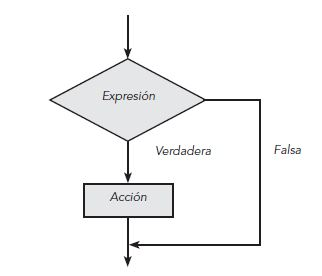
\includegraphics[scale=0.6]{flujoSeleccionSimple}
\end{center}
\end{frame}
%- - - - - - - - - - - - - - - - Slide 05 - - - - - - - - - - - - - - - - - -%
\begin{frame}[t]{Selección sencilla}
\textbf{Ejemplo:} Representar la superación de un examen (Nota >= 5, Aprobado).\\
\vspace{2mm}
\begin{center}
	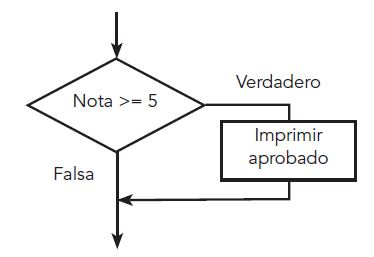
\includegraphics[scale=0.5]{flujoEjemploSeleccionSimple}
\end{center}
\end{frame}

%- - - - - - - - - - - - - - - - Slide 06 - - - - - - - - - - - - - - - - - -%
\begin{frame}[fragile]{Selección sencilla}
\lstinputlisting[style=customc]{codigos/seleccion/ejemploSeleccionSimple.c}
\end{frame}


% *******************************************************************************
% *							SELECCIÓN DOBLE										*
% *******************************************************************************

%- - - - - - - - - - - - - - - - Slide 07 - - - - - - - - - - - - - - - - - -%
\begin{frame}{Selección doble}
En este formato la sentencia \textbf{if} tiene la siguiente sintaxis:\\
\vspace{5mm}
\begin{columns}
	\begin{column}{0.33 \textwidth}
			\begin{block}{\textit{if} (Expresión)}
		Expresión lógica que determina la acción a ejecutar
		\end{block}	
	\end{column}
	\begin{column}{0.33 \textwidth}
		\begin{block}{Accion$ _{1} $}
			Acción que se realiza si la expresión lógica es verdadera.
		\end{block}	
	\end{column}
	\begin{column}{0.33 \textwidth}
		\begin{block}{\textit{else} Accion$ _2 $}
			Acción que se ejecuta si la expresión lógica es falsa.
		\end{block}
	\end{column}
\end{columns}
\end{frame}

%- - - - - - - - - - - - - - - - Slide 08 - - - - - - - - - - - - - - - - - -%
\begin{frame}{Selección doble}
Acción$ _{1} $ y Acción$ _{2} $, son individualmente, o bien una única instrucción que termina en
un punto y coma (;) o un grupo de instrucciones encerradas entre llaves.\\
\vspace{2mm}
Si \textit{Expresión} es verdadera, se ejecuta \textit{Acción$ _{1} $} y en caso contrario se ejecuta \textit{Acción$ _{2} $}
\begin{center}
	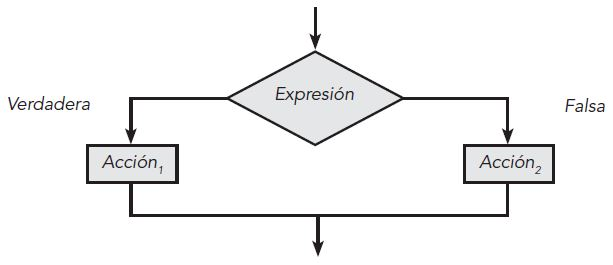
\includegraphics[width=0.7\linewidth]{figs/flujoSeleccionDoble}
\end{center}
\end{frame}

%- - - - - - - - - - - - - - - - Slide 09 - - - - - - - - - - - - - - - - - -%
\begin{frame}[fragile]{Selección doble}
\textbf{Ejemplo:} Calcular el mayor de dos números leídos del teclado y visualizarlo en pantalla.
%\begin{lstlisting}
%#include<stdio.h>
%
%int main(void)
%{
%    int x, y;
%    printf("Ingrese el primer valor: ");
%}
%\end{lstlisting}
\lstinputlisting[style=customc]{codigos/seleccion/ejemploSeleccionDoble.c}
\end{frame}

% *******************************************************************************
% *							SELECCIÓN MULTIPLE									*
% *******************************************************************************
%- - - - - - - - - - - - - - - - Slide 10 - - - - - - - - - - - - - - - - - -%
\begin{frame}[t, fragile]{Selección Multiple}
	Una sentencia \textbf{if} es anidada cuando la sentencia de la rama verdadera o la rama falsa es a su vez una sentencia if. Una sentencia \textbf{if} anidada se puede utilizar para implementar decisiones con varias alternativas o multialternativas.
	\begin{columns}
		\begin{column}{0.40 \textwidth}
		  \centering
			{\LARGE SINTAXIS:}
		\end{column}
		\begin{column}{0.40 \textwidth}
            \vspace{1.5mm}
			\begin{lstlisting}
if(condición_1)
    sentencia_1
else if(condicion_2)
    sentencia_2
    .
    .
else if(condicion_n-1)
    sentencia_n-1
else
    sentencia_n
\end{lstlisting}
		\end{column}	
	\end{columns}
\end{frame}

%- - - - - - - - - - - - - - - - Slide 10 - - - - - - - - - - - - - - - - - -%
\begin{frame}[c]{Selección Multiple}
La sentencia \textbf{switch} es una sentencia que se utiliza para seleccionar una de múltiples alternativas. Es especialmente útil cuando la selección se basa en el valor de una variable simple o de una expresión simple denominada \textbf{\textit{expresión de control}} o \textbf{\textit{selector}}. El valor de esta expresión puede ser de tipo \textit{\textbf{int}} o \textbf{\textit{char}}, pero no de tipo float ni double.
\end{frame}

%- - - - - - - - - - - - - - - - Slide 11 - - - - - - - - - - - - - - - - - -%
\begin{frame}[fragile]{Selección Multiple}
\centering
{\LARGE SINTAXIS}
    \begin{lstlisting}
switch (selector)
{
    case etiqueta1 : sentencias1;
    case etiqueta2 : sentencias2;
    .
    .
    case etiquetan : sentenciasn;
    default: sentencias; /* opcional */
}
\end{lstlisting}
\end{frame}


%- - - - - - - - - - - - - - - - Slide 12 - - - - - - - - - - - - - - - - - -%
\begin{frame}[t]{Selección Multiple}
\hspace{5mm}La expresión de control o \textbf{selector} se evalúa y se compara con cada una de las etiquetas de \textbf{case}. Cada etiqueta es un valor único, constante y cada etiqueta debe tener un valor diferente de los otros.\\
\hspace{5mm}Si el valor de la expresión selector es igual a una de las etiquetas case, por ejemplo, etiqueta1, entonces
la ejecución comenzará con la primera sentencia de la secuencia y continuará hasta que se encuentre el final de la sentencia de control switch, o hasta encontrar la sentencia \textbf{break}.\\
\hspace{5mm}Típicamente después de cada bloque se sitúa la sentencia \textbf{break }como última sentencia del bloque. La sentencia \textbf{break} hace que siga la ejecución en la siguiente sentencia al switch.
\end{frame}

%- - - - - - - - - - - - - - - - Slide 13 - - - - - - - - - - - - - - - - - -%
\begin{frame}[c,fragile]{Selección Multiple}
\centering
SINTAXIS CON break
\begin{lstlisting}
switch (selector)
{
    case etiqueta1 : sentencias1;
    break;
    case etiqueta2 : sentencias2;
    break;
    .
    .
    .
    case etiquetan :sentenciasn;
    break;
    default: sentenciasd; /* opcional */
}
\end{lstlisting}
\end{frame}

%- - - - - - - - - - - - - - - - Slide 14 - - - - - - - - - - - - - - - - - -%
\begin{frame}[c,fragile]{Selección Multiple}
\centering
Elección de tres opciones y un valor en forma predeterminada.
\begin{lstlisting}
switch (opcion)
{
    case 0:
        printf("Cero!");
        break;
    case 1:
        printf("Uno!");
        break;
    case 2:
        printf("Dos!");
        break;
    default:
        printf("Fuera de rango");
}
\end{lstlisting}
\end{frame}


%- - - - - - - - - - - - - - - - Slide 15 - - - - - - - - - - - - - - - - - -%
\begin{frame}[c,fragile]{Selección Multiple}
\centering
Selección múltiple, tres etiquetas ejecutan la misma sentencia.
\begin{lstlisting}
switch (opcion)
{
    case 0:
    case 1:
    case 2:
        printf("Menor de 3");
        break;
    case 3:
        printf("Igual a 3");
        break;
    default:
        printf("Mayor que 3");
}
\end{lstlisting}
\end{frame}


%- - - - - - - - - - - - - - - - Slide 16 - - - - - - - - - - - - - - - - - -%
\begin{frame}[fragile]{Selección Multiple}
Comparación de las sentencias if-else-if y switch. Se necesita saber si un determinado
carácter car es una vocal. Solución con if-else-if.
\vspace{2mm}
    \begin{columns}
        \begin{column}{0.4 \textwidth}
            \begin{lstlisting}[basicstyle=\ttfamily\tiny]
if((car=='a')||(car=='A'))
   printf("%c es una vocal\n",car);
else if((car=='e')||(car=='E'))
   printf("%c es vocal\n",car);
else if((car=='i')||(car=='I'))
   printf("%c es vocal\n",car);
else if((car=='o')||(car=='O'))
   printf("%c es vocal\n",car);
else if((car=='u')||(car=='U'))
   printf("%c es vocal\n",car);
else
   printf("%c no es vocal\n",car);
\end{lstlisting}
        \end{column}
        \begin{column}{0.5 \textwidth}
            \begin{lstlisting}[basicstyle=\ttfamily\tiny]
switch (car)
{
    case 'a': case 'A':
    case 'e': case 'E':
    case 'i': case 'I':
    case 'o': case 'O':
    case 'u': case 'U':
        printf("%c es una vocal\n",car);
        break;
    default:
       printf("%c no es una vocal\n",car);
}
\end{lstlisting}
        \end{column}
    \end{columns}

\end{frame}


%\begin{frame}[c]{Selección sencilla}
%La estructura selectiva \textbf{SI - ENTONCES} permite que el flujo de datos siga por un camino específico si se cumple una condición o conjunto de condiciones. \\
%\vspace*{2mm}
%Si al evaluar la condición (o condiciones) el resultado es verdadero, entonces se ejecutan un conjunto de operaciones. \\
%\vspace*{2mm}
%Luego, se continúa con la secuencia normal del flujo.\\
%\vspace{28mm}
%\tiny Battistutti, O. C. (2005). Metodología de la programación: Algoritmos, diagramas de flujo y programas (3rd ed.). México, D.F.: Alfaomega.
%\end{frame}


%- - - - - - - - - - - - - - - - Slide 04 - - - - - - - - - - - - - - - - - -%
%\begin{frame}[c]{Diagrama de flujo de la selección sencilla}
%\vspace*{4mm}
%\begin{center}
%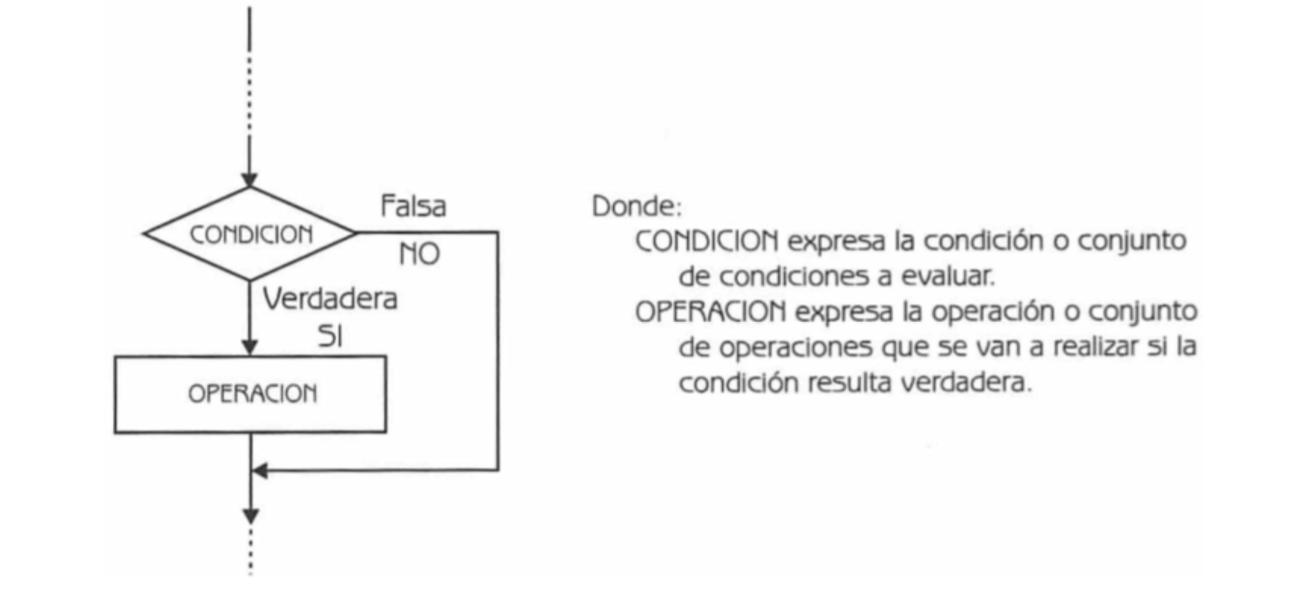
\includegraphics[scale=0.45]{figs/SeleccionSencillaDF.png}
%\end{center}
%\vspace*{-6mm}
%\tiny Battistutti, O. C. (2005). Metodología de la programación: Algoritmos, diagramas de flujo y programas (3rd ed.). México, D.F.: Alfaomega.
%\end{frame}


%- - - - - - - - - - - - - - - - Slide 05 - - - - - - - - - - - - - - - - - -%
%\begin{frame}[fragile, c] \frametitle{Estructura de la selección sencilla}
%\begin{lstlisting}
%...
%if(CONDICION)
%{
%    OPERACION
%}
%...
%\end{lstlisting}
%\vspace*{35mm}
%%\tiny Aguilar, L. J., & Martínez, I. Z. (2010). Programación en C: Metodología, algoritmos y estructura de datos. Madrid: McGraw-Hill.
%\end{frame}


%- - - - - - - - - - - - - - - - Slide 06 - - - - - - - - - - - - - - - - - -%



%- - - - - - - - - - - - - - - - Slide 07 - - - - - - - - - - - - - - - - - -%



%- - - - - - - - - - - - - - - - Slide 08 - - - - - - - - - - - - - - - - - -%



%- - - - - - - - - - - - - - - - Slide 09 - - - - - - - - - - - - - - - - - -%
